%!TEX root = ../main.tex

\begin{frame}
\frametitle{Transactions and Concurrency Control}
\begin{itemize}
\item InfiniteGraph supports two transaction models
\begin{description}
    \item[Standard Ingest] ACID transactions
    \item[Accelerated Ingest] Eventual consistency
\end{description}
\item \emph{Ingest} means updating the graph
\end{itemize}
\end{frame}

\begin{frame}
\frametitle{Standard Ingest}
\begin{itemize}
    \item Offers full ACID transactions
    \begin{itemize}
        \item Thus CP and PC/EC
    \end{itemize}
    \item Page-level read/write locking, no further details given
    \item Immediate consistency after commit
\end{itemize}
\end{frame}

\begin{frame}
\frametitle{Advanced Ingest}
\begin{itemize}
    \item Few information on implementation
    \item Offers "eventual consistency"
    \item No definite information on CAP and PAC/ELC:
    \begin{itemize}
        \item \begin{quote}
            However, we do plan to offer replication with eventual 
            consistency in the future.  The goal is to offer consistency, 
            availability, and partition tolerance (CAP).\footnote{\url{https://groups.google.com/forum/?fromgroups\#!msg/infinitegraph/X-YkLwKjHXs/R07gypaSknQJ}}
        \end{quote}
        \item P?/EL because of eventual consistency
    \end{itemize}
\item Transactions still supported for rollback
\item No information given on
\begin{itemize}
    \item How conflicts are handled
    \item What kind of eventual consistency
\end{itemize}
\end{itemize}
\end{frame}

\begin{frame}
    \frametitle{Advanced Ingest}
\begin{figure}[h]
    \centering
        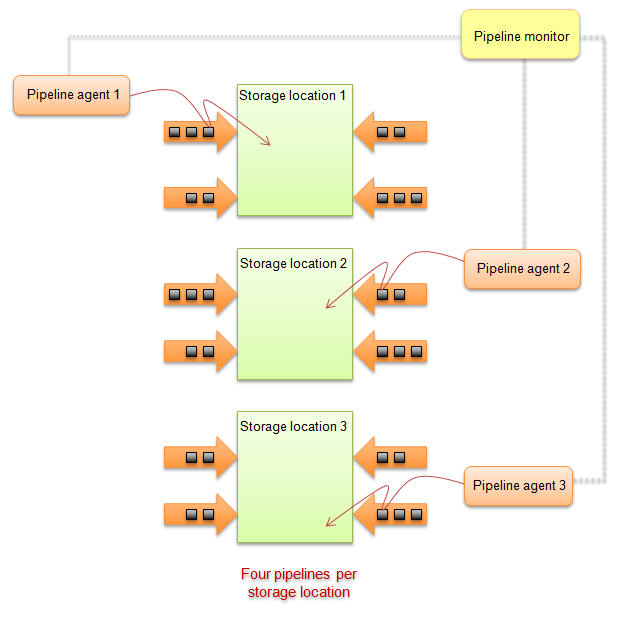
\includegraphics[width=.7\textwidth]{images/acceleratedIngest.jpg}
    \caption{caption}
    \label{fig:images_acceleratedIngest}
\end{figure}
\end{frame}